%%%%%%%%%%%%%%%%%%%%%%%%
%
% $Autor: Hemanth Jadiswami Prabhakaran $
% $Datum: 2025-06-30 11:03:19Z $
% $Pfad: GitHub/BA25-01-Time-Series/report/Contents/en/gitHubActions.tex $
% $Version: 1 $
%
% $Project: BA25-Time-Series $
%
%%%%%%%%%%%%%%%%%%%%%%%%

\chapter{GitHub Actions: Automating LaTeX Compilation }


\section{Introduction}


In the contemporary landscape of academic and technical writing, the automation of document compilation has become increasingly crucial for maintaining consistency, reproducibility, and efficiency in scholarly workflows. GitHub Actions, a continuous integration service launched by GitHub in 2018, represents a significant advancement in continuous integration and continuous deployment (CI/CD) technologies, offering researchers and academics a powerful platform for automating their LaTeX compilation processes \cite{Chacon:2014, Kim:2016, GitHub:2023}.

The integration of version control systems with automated build processes has transformed how academic documents are developed and maintained. As noted by Humble and Farley in their seminal work on continuous delivery \cite{Humble:2010}, automation reduces human error, ensures reproducibility, and accelerates the feedback loop in document development. This principle extends naturally to LaTeX document compilation, where complex dependencies, multiple compilation passes, and bibliography processing can benefit significantly from automation.

GitHub Actions provides a cloud-based execution environment that responds to repository events, enabling authors to automatically compile their LaTeX documents upon each commit or pull request. This approach aligns with the principles of Infrastructure as Code (IaC), where the build process itself becomes versionable, shareable, and reproducible \cite{Morris:2016}. 

In the context of the Walmart Sales Forecasting project, maintaining an automated document pipeline ensures reliable delivery of reproducible results and proper version control. For academic projects involving multiple collaborators or requiring frequent document updates, this automation becomes not merely convenient but essential for maintaining document integrity and consistency.

\section{GitHub Actions Architecture for LaTeX Projects}


\subsection{Core Concepts and Components}

GitHub Actions operates on an event-driven architecture, where workflows respond to repository events such as pushes or pull requests. Each workflow comprises one or more jobs, which are executed on virtual machines ('runners') and consist of sequential steps. These steps may involve setting up the environment, compiling documents, and handling outputs \cite{GitHub:2023}.

In the context of LaTeX automation, these workflows typically consist of:

\begin{itemize}
	\item \textbf{Triggers}: Events that initiate the workflow, such as pushes to the main branch or pull request creation
	\item \textbf{Jobs}: Discrete units of work that execute on virtual machines (runners)
	\item \textbf{Steps}: Individual tasks within a job, such as installing dependencies or compiling documents
	\item \textbf{Artifacts}: Output files (e.g., compiled PDFs) that are preserved after workflow completion
\end{itemize}

The workflow configuration is defined in YAML format, stored within the repository's \texttt{.github/workflows/} directory. This approach ensures that the build configuration is version-controlled alongside the document source, adhering to the principle of configuration as code \cite{Humble:2010}.

\subsection{LaTeX-Specific Considerations}

Automating LaTeX compilation presents unique challenges compared to traditional software builds. LaTeX documents often require:

\begin{enumerate}
	\item Multiple compilation passes to resolve cross-references
	\item Bibliography processing using tools like BibTeX or Biber
	\item Specific font and package dependencies
	\item Handling of auxiliary files and intermediate build artifacts
\end{enumerate}

Our implementation addresses these challenges through a systematic approach that mirrors the manual compilation process while adding robustness through error handling and conditional logic.

\section{Implementation: Multi-Document LaTeX Compilation Pipeline}


Our GitHub Actions workflow automates the compilation of four distinct LaTeX document types: a comprehensive manual, a scientific poster, a detailed report, and a presentation. Each document type requires specific compilation strategies and dependency management.

\subsection{Workflow Configuration and Triggers}

The workflow begins with event configuration:

\begin{lstlisting}[breaklines=true][ caption={Workflow triggers configuration}, label={lst:triggers}]
	name: Build Walmart LaTeX PDFs
	
	on:
	push:
	branches:
	- main
	pull_request:
\end{lstlisting}

This configuration ensures that documents are compiled both when changes are merged to the main branch and during the review process for pull requests, providing immediate feedback on document compilation status.

\subsection{Environment Setup}

The LaTeX compilation environment requires careful configuration to ensure all necessary packages and tools are available. The comprehensive package list includes specialized packages for scientific writing, multilingual support, and advanced graphics processing:

\begin{lstlisting}[breaklines=true][ caption={LaTeX environment installation}, label={lst:environment}]
	- name: Install LaTeX environment
	run: |
	sudo apt-get update
	sudo apt-get install -y \
	texlive-xetex \
	texlive-fonts-recommended \
	texlive-latex-recommended \
	texlive-latex-extra \
	texlive-bibtex-extra \
	texlive-science \
	texlive-lang-german \
	texlive-fonts-extra \
	texlive-pictures \
	biber
\end{lstlisting}

The inclusion of \texttt{texlive-lang-german} accommodates potential multilingual requirements in collaborative academic environments, while \texttt{texlive-science} provides specialized mathematical and scientific notation packages commonly required in technical documentation.

\subsection{Document-Specific Compilation Strategies}

\subsubsection{Manual Compilation}

The manual compilation demonstrates the standard three-pass compilation process with bibliography processing:

\begin{lstlisting}[breaklines=true][ caption={Manual compilation process}, label={lst:manual}]
	- name: Compile Manual
	working-directory: ./Manual
	run: |
	xelatex -interaction=nonstopmode WalmartSalesForecastingManual.tex
	biber WalmartSalesForecastingManual
	xelatex -interaction=nonstopmode WalmartSalesForecastingManual.tex
	xelatex -interaction=nonstopmode WalmartSalesForecastingManual.tex
\end{lstlisting}

The \texttt{-interaction=nonstopmode} flag ensures that compilation continues despite non-fatal errors, preventing the workflow from hanging on user input prompts.

\subsubsection{Report Compilation with Conditional Bibliography Processing}

The report compilation showcases advanced error handling and conditional logic for bibliography processing, accommodating varying bibliography backends depending on collaborators' preferences or legacy documents:

\begin{lstlisting}[breaklines=true][ caption={Conditional bibliography processing}, label={lst:bibprocessing}]
	- name: Compile Report
	working-directory: ./report
	run: |
	echo "Running first XeLaTeX pass..."
	xelatex -interaction=nonstopmode WalmartSalesForecastingReport.tex
	
	if [ -f "WalmartSalesForecastingReport.bcf" ]; then
	echo "Using Biber backend"
	biber WalmartSalesForecastingReport
	elif [ -f "WalmartSalesForecastingReport.aux" ]; then
	echo "Using BibTeX8 backend"
	if grep -q "\\citation" WalmartSalesForecastingReport.aux; then
	bibtex8 WalmartSalesForecastingReport
	else
	echo "No citations found in AUX file"
	fi
	fi
	
	xelatex -interaction=nonstopmode WalmartSalesForecastingReport.tex
	xelatex -interaction=nonstopmode WalmartSalesForecastingReport.tex
\end{lstlisting}

This approach demonstrates defensive programming principles, accommodating different bibliography backends and handling cases where no citations exist.

\subsection{Artifact Management}

Each compiled document is preserved as a workflow artifact:

\begin{lstlisting}[breaklines=true][ caption={Artifact upload configuration}, label={lst:artifacts}]
	- name: Upload Report PDF
	uses: actions/upload-artifact@v4
	with:
	name: WalmartSalesForecastingReport-pdf
	path: report/WalmartSalesForecastingReport.pdf
\end{lstlisting}

This ensures that compiled PDFs are accessible for download even after the workflow completes, facilitating distribution and review.

\section{Workflow Architecture Visualization}
\label{sec:visualization}

The following diagram illustrates the complete workflow architecture for documents compiled using XeLaTeX with bibliography support:

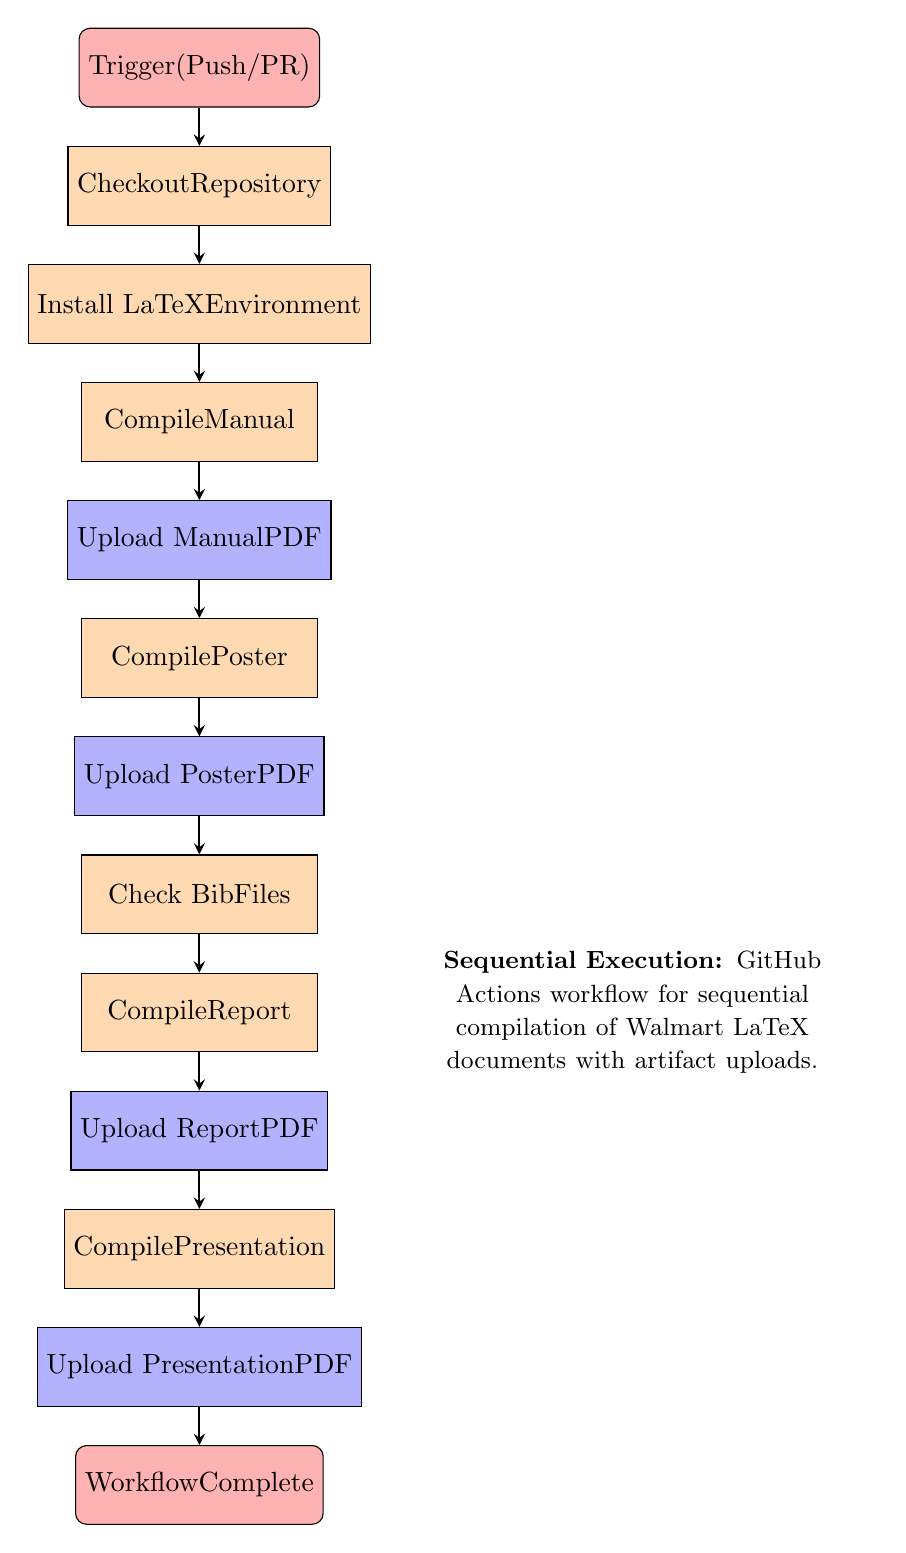
\begin{tikzpicture}[node distance=1.5cm,
	every node/.style={minimum width=3cm, minimum height=1cm, text centered},
	startstop/.style={rectangle, rounded corners, draw=black, fill=red!30},
	process/.style={rectangle, draw=black, fill=orange!30},
	io/.style={rectangle, draw=black, fill=blue!30},
	arrow/.style={thick,->,>=stealth}]
	
	% Start
	\node (start) [startstop] {Trigger\\(Push/PR)};
	
	% Setup
	\node (checkout) [process, below of=start] {Checkout\\Repository};
	\node (latex) [process, below of=checkout] {Install LaTeX\\Environment};
	
	% Manual
	\node (manual) [process, below of=latex] {Compile\\Manual};
	\node (manual_upload) [io, below of=manual] {Upload Manual\\PDF};
	
	% Poster
	\node (poster) [process, below of=manual_upload] {Compile\\Poster};
	\node (poster_upload) [io, below of=poster] {Upload Poster\\PDF};
	
	% Report
	\node (report_check) [process, below of=poster_upload] {Check Bib\\Files};
	\node (report) [process, below of=report_check] {Compile\\Report};
	\node (report_upload) [io, below of=report] {Upload Report\\PDF};
	
	% Presentation
	\node (presentation) [process, below of=report_upload] {Compile\\Presentation};
	\node (pres_upload) [io, below of=presentation] {Upload Presentation\\PDF};
	
	% End
	\node (end) [startstop, below of=pres_upload] {Workflow\\Complete};
	
	% Sequential arrows
	\draw [arrow] (start) -- (checkout);
	\draw [arrow] (checkout) -- (latex);
	\draw [arrow] (latex) -- (manual);
	\draw [arrow] (manual) -- (manual_upload);
	\draw [arrow] (manual_upload) -- (poster);
	\draw [arrow] (poster) -- (poster_upload);
	\draw [arrow] (poster_upload) -- (report_check);
	\draw [arrow] (report_check) -- (report);
	\draw [arrow] (report) -- (report_upload);
	\draw [arrow] (report_upload) -- (presentation);
	\draw [arrow] (presentation) -- (pres_upload);
	\draw [arrow] (pres_upload) -- (end);
	
	% Add a note
	\node [text width=6cm, right of=report, xshift=4cm] {\small \textbf{Sequential Execution:} GitHub Actions workflow for sequential compilation of Walmart LaTeX documents with artifact uploads.};
	
\end{tikzpicture}


\section{Customizing the Workflow for Other Projects}
\label{sec:adaptation}

\subsection{Essential Modifications}

To adapt this workflow for your own LaTeX projects, consider the following modifications:

\subsubsection{1. Document Structure}
Update the directory paths and filenames to match your project structure:
\begin{lstlisting}[breaklines=true]
	working-directory: ./your-document-directory
	run: |
	xelatex -interaction=nonstopmode your-document-name.tex
\end{lstlisting}

\subsubsection{2. LaTeX Engine Selection}
Choose the appropriate LaTeX engine based on your document requirements:
\begin{itemize}
	\item \texttt{pdflatex}: Standard engine for most documents
	\item \texttt{xelatex}: Required for Unicode support and system fonts
	\item \texttt{lualatex}: Modern engine with Lua scripting capabilities
\end{itemize}

\subsubsection{3. Package Dependencies}
Customize the package installation based on your document's requirements. For minimal installations:
\begin{lstlisting}[breaklines=true]
sudo apt-get install -y texlive-latex-base texlive-latex-recommended
\end{lstlisting}

\subsection{Common Pitfalls and Solutions}

\subsubsection{Bibliography File Detection}
Ensure bibliography files are in the correct location relative to your main document. The workflow includes debugging steps:
\begin{lstlisting}[breaklines=true]
	- name: Check bibliography files
	run: |
	echo "Checking for bibliography files..."
	ls -la *.bib || echo "No .bib files found"
\end{lstlisting}

\subsubsection{Memory Limitations}
Large documents may exceed GitHub Actions' memory limits (approximately 7 GB RAM) or timeout constraints (6 hours maximum execution time). Consider:
\begin{itemize}
	\item Splitting large documents into smaller components
	\item Using draft mode for intermediate compilations
	\item Implementing incremental builds
\end{itemize}

\subsubsection{Compilation Timeouts}
GitHub Actions enforces time limits on workflow execution. Optimize compilation time by:
\begin{itemize}
	\item Caching LaTeX installations between runs
	\item Parallelizing independent document compilations
	\item Using faster compilation modes where appropriate
\end{itemize}

\subsection{Advanced Features}

Consider implementing these advanced features for enhanced functionality:

\subsubsection{1. Conditional Compilation}
Compile only changed documents using Git diff with updated syntax:
\begin{lstlisting}[breaklines=true]
	- name: Detect changed files
	id: changed-files
	run: |
	echo "docs=$(git diff --name-only HEAD^ HEAD | grep '\.tex$')" >> "$GITHUB_OUTPUT"
\end{lstlisting}

\subsubsection{2. Version Tagging}
Automatically tag compiled PDFs with version information:
\begin{lstlisting}[breaklines=true]
	- name: Tag PDF with version
	run: |
	VERSION=$(git describe --tags --always)
	mv output.pdf output-${VERSION}.pdf
\end{lstlisting}

\subsubsection{3. Notification Integration}
Add notifications for compilation failures using reusable GitHub Actions:
\begin{lstlisting}[breaklines=true]
	- name: Notify on failure
	if: failure()
	uses: actions/github-script@v6
	with:
	script: |
	github.rest.issues.createComment({
		issue_number: context.issue.number,
		body: 'LaTeX compilation failed. Check the logs.'
	})
\end{lstlisting}

For enhanced functionality, consider utilizing marketplace actions such as \texttt{upload-artifact}, \texttt{github-script}, and notification integrations available through the GitHub Actions marketplace.

\section{Conclusion}


The implementation of GitHub Actions for LaTeX document automation represents a significant advancement in academic workflow management. By automating the compilation process, researchers can focus on content creation while ensuring consistent, reproducible document generation. The workflow presented here demonstrates how modern CI/CD practices can be successfully applied to academic document preparation, reducing manual effort and minimizing compilation errors.

The flexibility of GitHub Actions allows for extensive customization, enabling researchers to adapt the workflow to their specific requirements while maintaining the benefits of automation. As academic collaboration increasingly relies on digital platforms, such automation becomes not merely a convenience but a necessity for efficient scholarly communication.

Future enhancements might include integration with reference management systems, automated quality checks for LaTeX documents, and deployment to institutional repositories. The foundation provided by this workflow serves as a starting point for such advanced automation scenarios.

